\documentclass[border=2pt]{standalone}
\usepackage{tikz}
\usetikzlibrary{shapes.geometric,positioning,arrows.meta}
\begin{document}
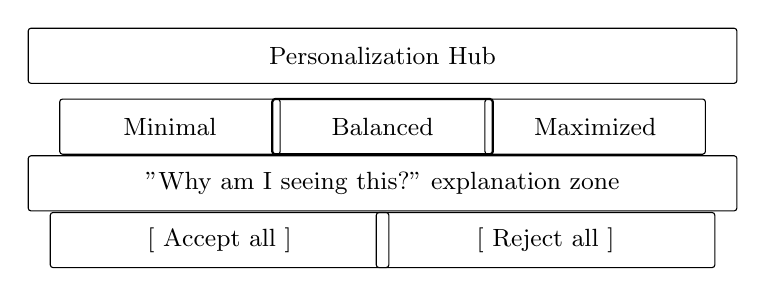
\begin{tikzpicture}[
  box/.style={draw, rounded corners=1pt, minimum height=0.7cm, font=\small},
  scale=0.9
]
\node[box, minimum width=9cm] (h) at (0,4) {Personalization Hub};
\node[box, minimum width=2.8cm] (t1) at (-3,3) {Minimal};
\node[box, minimum width=2.8cm, thick] (t2) at (0,3) {Balanced};
\node[box, minimum width=2.8cm] (t3) at (3,3) {Maximized};
\node[box, minimum width=9cm] (why) at (0,2.2) {"Why am I seeing this?" explanation zone};
\node[box, minimum width=4.3cm] (a) at (-2.3,1.4) {[ Accept all ]};
\node[box, minimum width=4.3cm] (r) at (2.3,1.4) {[ Reject all ]};
\end{tikzpicture}
\end{document}
